\documentclass[12pt]{article}
\usepackage[T1]{fontenc}
\usepackage[latin9]{luainputenc}
\usepackage{geometry}
\geometry{verbose,tmargin=0.8in,bmargin=0.8in,lmargin=0.8in,rmargin=0.8in}
\usepackage{color}
\usepackage{babel}
\usepackage{float}
\usepackage{amsmath}
\usepackage{amsthm}
\usepackage{amssymb}
\usepackage{graphicx}
\usepackage{setspace}
\usepackage[authoryear]{natbib}
\onehalfspacing
\usepackage[unicode=true,pdfusetitle,
            bookmarks=true,bookmarksnumbered=false,bookmarksopen=false,
 breaklinks=false,pdfborder={0 0 1},backref=false,colorlinks=true]
 {hyperref}
\hypersetup{
 pdfborderstyle=,pdfborderstyle={},pdfborderstyle={},linkcolor=blue,urlcolor=blue,citecolor=blue,pdfstartview={FitH},hyperfootnotes=false}

\makeatletter


%%%%%%%%%%%%%%%%%%%%%%%%%%%%%% LyX specific LaTeX commands.
%% Because html converters don't know tabularnewline
\providecommand{\tabularnewline}{\\}

%%%%%%%%%%%%%%%%%%%%%%%%%%%%%% User specified LaTeX commands.
\usepackage{etex}
%\usepackage[round,longnamesfirst]{natbib}
\usepackage{amsfonts}
\usepackage{mathpazo}
\usepackage{hyperref}
\usepackage{xcolor}
\hypersetup{
	colorlinks,
	linkcolor={blue!75!black},
	citecolor={blue!75!black},
}
\usepackage{multimedia}
\usepackage{graphicx, color}
%\usepackage{pstricks,pst-node,fancybox,pst-text}
\usepackage{epsfig}
\usepackage{amsthm}
\usepackage{mathtools}
\usepackage{esint}
\usepackage{amssymb}
\usepackage{url}
\usepackage{graphicx,subfig}
\usepackage{relsize}
\usepackage{amsfonts}
\usepackage{fancyheadings}
\usepackage{float}
\usepackage{color}
\usepackage{mathrsfs}
\usepackage{setspace}
%\usepackage{lipsum}
%\usepackage{tikz}
\usepackage[mathscr]{euscript}
\usepackage{caption}
%\usepackage{subcaption}
\usepackage{pdflscape}
\usepackage{rotating}
\usepackage{booktabs}
%\usepackage[utf8]{inputenc}
\usepackage[T1]{fontenc}
\usepackage{geometry}
\newtheorem{thm}{Theorem}[section]
\newtheorem{cor}[thm]{Corollary}
\newtheorem{lem}[thm]{Lemma}
\newtheorem{prop}[thm]{Proposition}
\usepackage[bottom]{footmisc}

\newenvironment{definition}[1][Definition]{\begin{trivlist}
		\item[\hskip \labelsep {\bfseries #1}]}{\end{trivlist}}

\setlength{\topmargin}{-0.4in}
\setlength{\textheight}{8.85in}

%%  Edited to make stat review comments easier
\newif\ifStatReview% \StatReviewfalse
%%\StatReviewtrue    %   Show stat review comments
\StatReviewfalse    %   Ignore stat review comments
\ifStatReview
    \setlength{\oddsidemargin}{-0.2in}
    \setlength{\evensidemargin}{0.0in}
    \setlength{\textwidth}{6.0in}
    
    
    \usepackage{tikz}
    \let\oldmarginpar\marginpar
    % renew the \marginpar command to draw 
    % a node; it has a default setting which 
    % can be overwritten
    \renewcommand{\marginpar}[2][rectangle,draw,fill=yellow,rounded corners,text width=3.5cm]{%
            \oldmarginpar{%
            \tikz \node at (0,0) [#1]{#2};}%
            }
    \newcounter{statreview}
    \newenvironment{statreview}[1][]{\refstepcounter{statreview}\par\medskip
       \textbf{Stat Review~\thestatreview #1} \rmfamily}{\medskip}
  \else
    \setlength{\oddsidemargin}{-0.2in}
    \setlength{\evensidemargin}{0.0in}
    \setlength{\textwidth}{6.93in}
    \renewcommand{\marginpar}[2][]{}
\fi

\renewcommand{\baselinestretch}{1.44}

\usepackage{setspace}
\onehalfspacing

\@ifundefined{showcaptionsetup}{}{%
 \PassOptionsToPackage{caption=false}{subfig}}
\usepackage{subfig}
\makeatother


\begin{document}
\title{Title Goes Here!!!\thanks{Valdes-Bobes: University of Wisconsin.
		I thank [X] for helpful comments and discussions.}}
\author{Mitchell Valdes-Bobes}
\maketitle
\begin{abstract}
	We examine [X]
\end{abstract}
\thispagestyle{empty}

\pagebreak{}
This paper .... 


\section{Model of technological change \label{sec:model}}

In this section we present a simple model of the labor market with technological change....


\subsection{Model Overview \label{subsec:model_overview}}

In this Section [X]

When a worker and a firm are matched with one another, production occurs according to an "up-to-the task" production function (e.g., \citet{albrecht2002matching} and \citet{jarosch2019statistical}), which defines the output of the match to be,
\begin{align}
		f(h,z)=\begin{cases}
			z & h\ge z\\
			0 & \text{o.w.} \label{eq:prod_func}.
		\end{cases}
\end{align}
The production function in equation \ref{eq:prod_func} requires workers to have a minimum amount of human capital to produce with a given technology. We use the up to the task production function as it introduces a notion of skill requirements, based upon technology, to work in a given occupation.	
	
\section{Measuring technological change} \label{sec: measuring_tech_change}

In this section, we discuss of the construction of our measure of technological change using the Burning Glass database. We then discuss which occupations have been the most and least exposed to technological change and the characteristics of occupations that are associated with greater exposure to technological change. 

As an example of technological change, we examine the spread of computers and software within an occupation. We focus on computer and software requirements as our measure of technological change as innovation in the workplace commonly occurs via changes in software (e.g., \citet*{arora2013going} and \citet*{branstetter2019get}). Following \citet*{hershbein2018recessions}, we define a vacancy to contain a computer or software related skill if any of its reported skill requirements contain the keyword ``Computer'' or if any of the reported skill requirements are classified by Burning Glass as a software skill. We then measure for each occupation the share of vacancies in a given year that contain a computer or software related skill. Let $z_{o,t}$ denote the share of vacancies in occupation $o$ and year $t$ that contain a computer or software related skill. In our baseline analysis, we categorize occupations using 4-digit SOC codes as in \citet{hershbein2018recessions}, but show that our results are robust to alternative occupation classifications. 

To examine whether the share of vacancies in an occupation listing a computer or software requirement is informative about the use of computers and software in that occupation, we compare the estimates
from Burning Glass with data from O{*}NET. {O{*}NET asks individuals working in a given occupation as well as occupational experts to rate the level of knowledge needed in an occupation for a given set of skills/tasks and has been commonly used to measure the tasks performed in an occupation (e.g., \citet{acemoglu2011skills}). The level of knowledge is scored 0-7, with higher values indicating that a greater level of knowledge is required. Panel (a) of Figure \ref{fig:Technology Adoption by firms} compares the share of vacancies listing a computer skill requirement (\textit{y-axis}) to the level of computer knowledge recorded in O{*}NET (\textit{x-axis}) for each four-digit occupation.\footnote{We use vintage 15.1 of O*NET to measure computer usage by occupation (the O*NET variable is 2.C.3.a), which contains data collected between 2005 and 2010. We use this vintage as the midpoint of the data collection period aligns with the initial year of data from Burning Glass (2007).} The graph shows that our measure of computer and software requirements based on the skill content listed in online vacancies is highly correlated with the measure from O{*}NET. This finding suggests that the share of vacancies listing a computer or software requirement is informative about the use of computers and software in an occupation. % do we need to add a footnote/comment about why we do not just do the experiment w/ ONET. 

\begin{figure}[!tph]
	\caption{Technological Change by Occupation \label{fig:Technology Adoption by firms}}
	\begin{centering}
		\subfloat[Computer \& software req. by occ.]{
			\centering{}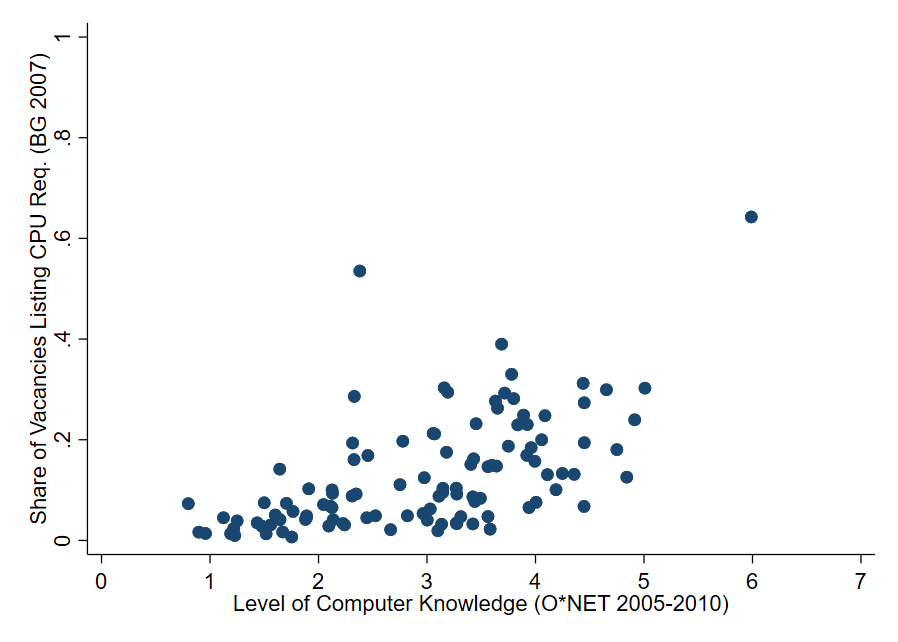
\includegraphics[width=8.5cm,height=8.5cm,keepaspectratio]{./images/scatter_level_BG_2007_ONET_15_1_pres_2021_08_18.png}}
		\subfloat[Changes in computer \& software req. by occ.]{
			\centering{}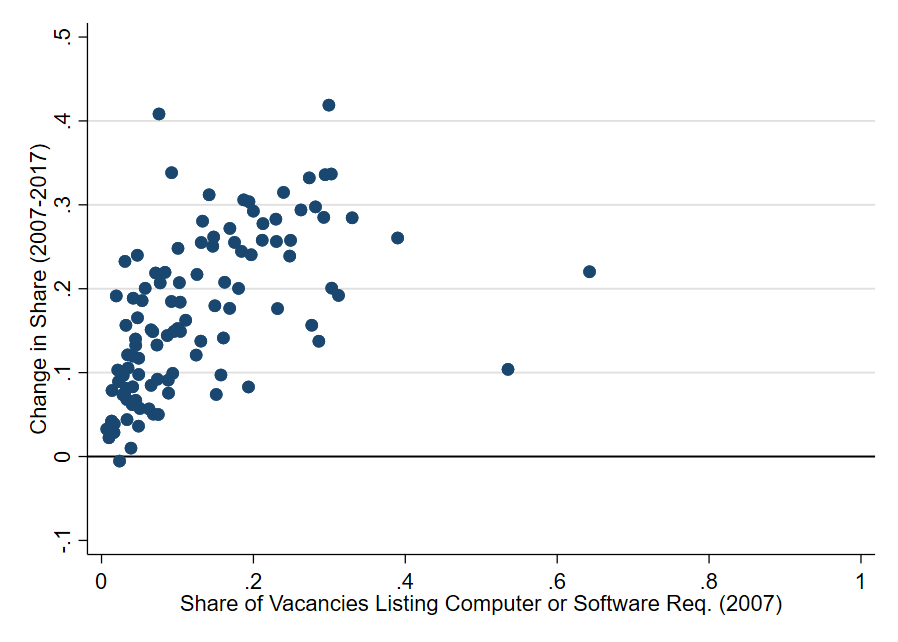
\includegraphics[width=8.5cm,height=8.5cm,keepaspectratio]{./images/scatter_chg_computer_by_initial_pres_2007_2021_08_18.png}}
		\par\end{centering}
	\emph{Notes: Panel (a) displays the level of knowledge in computers reported in O{*}NET (x-axis) and the share of vacancies listing a computer or software requirement by occupation as measured in the Burning Glass database in 2007 (y-axis). Panel (b) displays the share of vacancies listing a computer or software requirement by occupation in 2007 (x-axis), and the change in the share of vacancies listing a computer or software requirement between 2007 and 2017 (y-axis) as measured in the Burning Glass database. Occupations are measured using four-digit SOC codes.}\\	
\end{figure}
		
Given the measure $z_{o,t}$ of computer and software requirements in each occupation, we estimate technological change by measuring the change in the share of vacancies in a given occupation that contain a computer or software skill. Let $\varDelta z_{o}=z_{o,2017}-z_{o,2007}$ denote the change in the share of vacancies in occupation $o$ that list a computer or software skill requirement between $2007$ and $2017$. Panel (b) of Figure \ref{fig:Technology Adoption by firms} presents a scatter plot of computer and software requirements in 2007 (\textit{x-axis}) against the change in computer and software requirements between 2007 and 2017 by occupation (\textit{y-axis}). The scatter plot shows that nearly all occupations saw an increase in computer and software requirements between 2007 and 2017. Additionally, the scatter plot shows that there is significant heterogeneity in the adoption of computer and software requirements across occupations between 2007 and 2017. This heterogeneity in the adoption of computer and software requirements is critical for our identification of the impact of technological change on the outcomes of displaced workers, as we will compare the outcomes of workers displaced from occupations with large increases in computer and software requirements to the outcomes of workers displaced from occupations with a small increase in computer and software requirements. In the following subsection, we further examine which occupations have been more/less exposed to technological change as measures by changes in computer and software requirements over time. 
	

\subsection{Which occupations are changing computer \& software requirements}

In this section, we examine which occupations have been more exposed to technological change as measured by changes in computer and software requirements over time. We then examine the characteristics of occupations that are experiencing changes in computer and software requirements. 

Table \ref{tab: changes_by_occ} presents the 4-digit SOC occupations with the largest and smallest changes in computer and software requirements between 2007 and 2017.\footnote{In Appendix \ref{sec:chg_soc2} we present the change in computer and software requirements using broader 2-digit SOC occupation categories. }  The occupations with the largest increases in computer and software requirements include architects, engineers, advertising and marketing managers as well as protective service workers and their supervisors. Across these occupations we see different types of computer and software requirements being introduced. Among advertising and marketing managers there has been an increase in the demand for specific software packages and platforms. For instance Salesforce, Software as a Service (SaaS), and Google Analytics / Google Adwords are forms of software and platforms that were commonly listed in vacancies in 2017 but were rarely seen in 2007. Conversely, protective service jobs frequently include data entry by 2017 and job postings now list general computer skills and experience working with spreadsheets. 

In Appendix \ref{sec: robustness_occ_trends_ACS} we examine changes in employment and earnings structure by an occupation's exposure to technological change. We find that an occupation's exposure to technological change is not correlated with changes in employment share between 2007 and 2017. However, we find increased dispersion in earnings at both the top and bottom of the earnings distribution for occupations with greater exposure to technological change. 


% Table of top and bottom 10 occupations by change in CPU & software req. (2007-2017)
\begin{landscape}
	
\begin{table}[!tph]
	\caption{Changes in Computer and Software Requirements by Occupation \label{tab: changes_by_occ}}
	\begin{small} 
		\begin{centering}
			\begin{tabular}{lclccccc}
				\hline 
				\multicolumn{8}{c}{\emph{Panel A: Occupations with largest increase in computer \& software requirements} }\tabularnewline
				\hline 
				   &       &  & (1)  & (2)  & (3)  & (4)  & (5) \tabularnewline
				   &       &  & Chg. Computer  & Non-Routine & Routine  & Non-Routine  & Routine\tabularnewline
				Rank       & SOC-4  & Occupation  & Req. (2007-2017)  & Cognitive  & Cognitive & Manual  & Manual\tabularnewline
				\hline 
				1  & 1710  & Architects                                 & 0.419  & 1.603   & 0.657  & -0.187  & -0.285\tabularnewline
				2  & 3310  & Supervisors of protective service workers  & 0.408  & 1.036   & 0.160  & 1.845  & -0.250\tabularnewline
				3  & 3390  & Protective service workers                 & 0.338  & -0.656  & 1.160  & -0.966  & -1.036\tabularnewline
				4  & 1720  & Engineers - aerospace/biomedical/computer  & 0.337  & 0.323   & -0.468 & -1.587  & -0.868\tabularnewline
				5  & 4330  & Financial clerks                           & 0.336  & -0.705  & 1.878  & -0.633  & -0.311\tabularnewline
				6  & 1721  & Engineers - industrial/mechanical/nuclear  & 0.332  & 0.644   & -0.084 & -2.095  & -0.558\tabularnewline
				7  & 1520  & Mathematical science occupations           & 0.315  & 0.888   & -0.789 & -2.455  & -1.355\tabularnewline
				8  & 4750  & Oil, gas, and mining extraction workers    & 0.312  & -0.290  & 0.340  & 0.635  & 2.158\tabularnewline
				9  & 1120  & Advertising, marketing \& sales managers   & 0.306  & 1.815   & -1.540 & 0.419  & -1.506\tabularnewline
				10  & 2740  & Media and communication equipment workers & 0.304  & 0.097   & 0.605  & -0.235  & 1.112\tabularnewline
				\hline 
				\multicolumn{8}{c}{\emph{Panel B: Occupations with smallest increase in computer \& software requirements} }\tabularnewline
				\hline 
				&  &  & (1)  & (2)  & (3)  & (4)  & (5) \tabularnewline
				&  &  & Chg. Computer  & Non-Routine & Routine  & Non-Routine  & Routine\tabularnewline
				Rank  & SOC-4  & Occupation  & Req. (2007-2017)  & Cognitive  & Cognitive & Manual  & Manual\tabularnewline
				\hline 
				1  & 3990  & Personal care and service workers                & 0.044  & -0.641  & -2.490  & 0.894  & -1.245\tabularnewline
				2  & 3730  & Grounds maintenance workers                      & 0.042  & -1.010  & -2.386 & 0.091  & 2.112\tabularnewline
				3  & 5130  & Food processing workers                          & 0.041  & -0.832  & 0.150  & -0.736  & 1.281\tabularnewline
				4  & 3720  & Cleaners                                         & 0.039  & -1.992  & -1.330 & -1.225  & 0.647\tabularnewline
				5  & 3920  & Animal trainers and caretakers                   & 0.036  & -0.234  & -1.760 & 1.154  & -0.706\tabularnewline
				6  & 3520  & Cooks and food preparation workers               & 0.033  & -1.209  & -0.585 & -0.059  & 1.085\tabularnewline
				7  & 3590  & Restaurant attendants, dishwashers, hosts        & 0.029  & -1.758  & -1.242 & -0.041  & 0.762\tabularnewline
				8  & 4730  & Helpers, construction trades                     & 0.022  & -0.624  & -0.228 & -0.214  & 1.099\tabularnewline
				9  & 3530  & Food and drink servers                           & 0.010  & -1.040  & -0.394 & 0.210  & 0.214\tabularnewline
				10  & 5330  & Drivers - ambulance/bus/tractor trailors/taxis  & -0.005  & -1.207  & 0.476 & 2.487  & 1.323\tabularnewline
				\hline 
			\end{tabular}
			\par\end{centering}
		\emph{Note: Table presents the 10 occupations with the largest increase in computer and software requirements between 2007 and 2017 (Panel A), and the 10 occupations with the smallest increase (Panel B). Column (1) presents the change in the share of vacancies listing a computer and software requirements by occupation between 2007 and 2017 as measured in the Burning Glass data. Measures of the task content of an occupation presented in columns (2)-(5) are from \citet{acemoglu2011skills}. Occupations are classified using 4-digit SOC codes.} 
	\end{small} 
\end{table}

\end{landscape}

\pagebreak{}

% \bibliographystyle{chicago}
% \bibliography{references}

\pagebreak{}

\appendix

\section{Data and Estimation Details}

\section{Additional Results: Measure of Technological Change}

In this Appendix, we provide additional results on our measure of technological change based upon changes in computer and software requirements reported in the Burning Glass database. 

\subsection{Change in computer and software requirements by 2-digit SOC} \label{sec:chg_soc2}


\end{document}